% Lezione 3/2024-03-04
% - introduzione alla dinamica
% - prima e seconda legge
% - esercizi su moto uniformemente accelerato
% - accenni al concetto di forza e introduzione alla forza elastica con legge di hooke

% Lezione 4/2024-03-06
% - grafico orario: grafico nel quale un asse riporta lo spazio (una dimensione), mentre sull'altro il tempo
% - differenza tra SPOSTAMENTO e distanza
% - interpretazione grafica della velocità e accelerazione, con analisi di funzione

\chptr{Dinamica}
\marginpar{\minitoc}

\section{Recap}
\[ \overrightarrow{x} = \overrightarrow{x_0} + \overrightarrow{v}(t - t_0) \]
Semplificazioni in termini di variazioni, infinità.

\section{Leggi della dinamica}

Nella descrizione introduttiva del moto, non è stata analizzata alcuna causa del
fenomeno.

\subsection{La prima legge}

\vspace{8pt}
\begin{tcolorbox}[colback = red!30, colframe = red!30!black, title = {Prima legge della dinamica (legge di inerzia)}]
    Un corpo permane nel suo stato di \textit{quiete} o moto rettilineo uniforme
    finché non intervenga un \textit{agente esterno}.
\end{tcolorbox}
\vspace{5pt}

In altre parole, se nulla ``rompe le scatole'' al corpo, esso permanerà nel suo
stato di moto, naturalmente.

\vspace{8pt}
\begin{tcolorbox}[colback = yellow!30, colframe = yellow!30!black, title = {Sistema inerziale}]
    Sistema nel quale vale la prima legge della dinamica.
\end{tcolorbox}
\vspace{5pt}

\subsection{La seconda legge}
Quando l'agente esterno agisce sull'oggetto, l'effetto è un cambiamento nello
stato di moto di quell'oggetto. Ovvero, cambia la sua velocità. La variazione
della velocità nel tempo è chiamata \textbf{accelerazione}.

\[ \lim_{\Delta t \to 0} \frac{\Delta v}{\Delta t} = \frac{dv}{dt} = a \]

\vspace{8pt}
\begin{tcolorbox}[colback = red!30, colframe = red!30!black, title = {Seconda legge della dinamica}]
    \begin{align}
        \frac{|\overrightarrow{F}|}{|\overrightarrow{a}|} = \frac{F}{a} = m
    \end{align}
\end{tcolorbox}
\vspace{5pt}


Gli oggetti hanno inerzia, ovvero capacità di opporsi all'agire dell'agente
esterno. Questa capacità di opporsi è rappresentato da una quantità detta
massa (inerziale).

\subsection{Analisi dimensionale}
\[ [F] = [ma] = \left[m\cdot\frac{v}{t}\right] = \left[m\cdot\frac{l}{t^2}\right]  \]
\[ 1\text{ kg}\cdot\frac{\text{m}}{\text{s}^2} = \text{udm}\left[M\cdot\frac{L}{T^2}\right] = \text{udm}[F] = 1\text{ N} \]


\subsection{Molla e forza elastica}
\[ F \propto \Delta x \]

La forza che la molla esercita, essendo in opposizione alla direzione nella
quale la deformazione viene effettuata, corrisponde a:
\[ F_\textit{el} = -k\Delta x \]

\section{Forza agente sul moto}
Un blocco di massa $m = 10 \text{ kg}$ viaggia ad una velocità $v_i =
2 \text{ m/s}$. Una forza $F = 20 \text{ N}$ agisce sul blocco per
$T = 5 \text{ s}$. Quale velocità raggiungerà il blocco dopo $T$?.
Dopo $T$, la forza cessa di agire e il blocco viaggia a $v_f$ trovata
precedentemente. Includendo lo spazio percorso durante $T$ (e dunque il
tempo $T$), quanto tempo impiega il blocco a coprire $s_w = 2\text{ km}$
di distanza?

\begin{marginfigure}
    \centering
    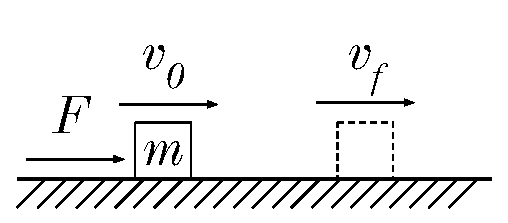
\includegraphics[width = \marginparwidth]{figures/scivola.pdf}
    \caption{Forza agente su una massa in moto}
\end{marginfigure}

Per rispondere al primo quesito, possiamo assumere un moto rettilineo
uniformemente accelerato durante l'intervallo $T$. Sappiamo che \[ a = \frac{F}{m} = \frac{dv}{dt} \]
Da cui possiamo esprimere la velocità in funzione del tempo (la velocità
iniziale la conosciamo già, ma assumiamo un tempo iniziale $t_0 = 0$):
\[ \frac{F}{m}dt = dv \to \int_{t_0}^{t}\frac{F}{m}dp = \int_{v_0}^{v}dw \to \frac{F}{m}\int_{0}^{t}dp = v - v_0 \to \frac{F}{m}t = v - v_0 \]
Dunque
\[ v(t) = v_0 + \frac{F}{m}t \]
Non ci manca che calcolare la velocità in corrispondenza di un $t_f = t_0 + \Delta t = 0 + T = T$:
\[ v(t_f) = v(T) = v_0 + \frac{F}{m}T \]

Nel secondo quesito, possiamo spezzare il problema in due parti: durante
l'azione della forza, la distanza percorsa ($s_a$) deve essere calcolata tenendo
conto del moto uniformemente accelerato, mentre nell'intervallo di tempo
successivo ($T_v$) il moto è semplicemente uniforme. Dalla seguente equazione,
possiamo ricavare $T_v$ ($T$ lo conosciamo già).
\[ s_w = s_a + s_v = s_a + v_fT_v = \int_{0}^{T}(v_0 + at)dp + v_fT_v = v_0T + \frac{1}{2}aT^2 + v_fT_v \]
Il tempo per percorrere $2\text{ km}$ è dunque:
\[ T_{2\text{ km}} = T + \frac{s_w - v_iT - \frac{F}{2m}T^2}{v_f} = T + \frac{s_w - v_iT - \frac{F}{2m}T^2}{v_i + \frac{F}{m}T} \]

\section{Lancio verso l'alto}
Si consideri la situazione mostrata in Figura \ref{lanciobasso}.
Durante la salita, l'oggetto rallenta a causa dell'accelerazione di gravità $g$.
Determiniamo la quota che l'oggetto raggiungerà.

\[ a = \frac{dv}{dt} \to dv = adt \to \int_{v_0}^{v}dw = \int_{t_0}^{t}adp \to v - v_0 = a\int_{t_0}^{t}dp \to v - v_0 = a(t - t_0) \]
Dunque
\[ v(t) = v_0 + a(t - t_0) = v_0 + at \]
Rallentando, si arriverà ad un istante $t_f$ nel quale l'oggetto avrà velocità
nulla:
\begin{marginfigure}
    \centering
    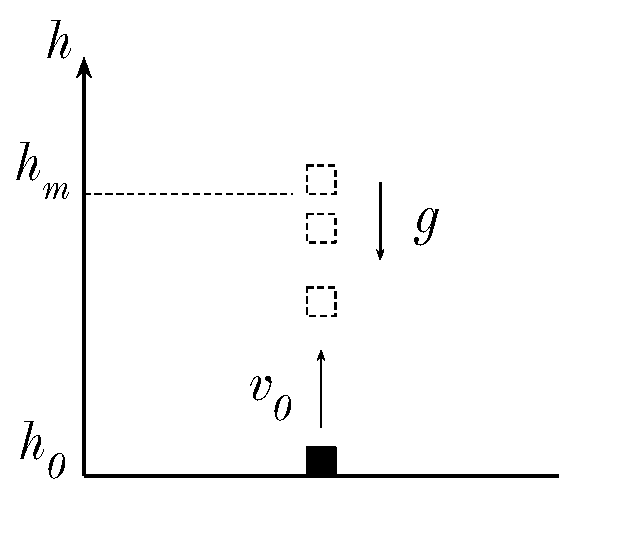
\includegraphics[width = \marginparwidth]{figures/greve.pdf}
    \caption{Lancio di un oggetto verso l'alto}
    \label{lanciobasso}
\end{marginfigure}
\[ v(t_f) = 0 \to v_0 + at_f = 0 \]
Non disponiamo tuttavia del tempo, ma possiamo avvalerci della legge oraria
che descrive la distanza percorsa:
\[ v(t) = \frac{dh}{dt} \to \int_{h_0}^{h}dk = \int_{t_0}^{t}v(t)dp \to h - h_0 = \int_{t_0}^{t}(v_0 + ap)dp \]
\[ h - h_0 = v_0\int_{t_0}^{t}dp + a\int_{t_0}^{t}pdp \to h - h_0 = v_0t + \frac12 at^2 \]
Da cui:
\[ h(t) = h_0 + v_0t + \frac12 at^2 = v_0t + \frac12 at^2 \]
Abbiamo quindi ottenuto la quota in funzione del tempo, che possiamo ricavare
dall'equazione $v_0 + at_f = 0 \to t_f = -\frac{v_0}{a}$.
\[ h(t_f) = v_0t_f + \frac12 at_{f}^2 =  -\frac{v_0^2}{a} + \frac{1}{2}a\frac{v_0^2}{a^2} = -\frac{v_0^2}{a} + \frac{v_0^2}{2a} = -\frac{v_0^2}{2a} \]
Sapendo che $a = -|g|$, la quota massima $h_m$ raggiunta è:
\[ h_m = \frac{v_0^2}{2|g|} \]

%%%%%%%%%%%%%%%%%%%%%%%%%%%%%%%%%%%%%%%%%%%%%%%%%%%%%%%%%%%%%%%%%

\subsection*{Spostamento}
\[ \Delta\overrightarrow{s} = \overrightarrow{s}_f - \overrightarrow{s}_i \]


\subsection{La terza legge}
\vspace{8pt}
\begin{tcolorbox}[colback = red!30, colframe = red!30!black, title = {Terza legge della dinamica}]

\end{tcolorbox}
\vspace{5pt}



\vspace{8pt}
\begin{tcolorbox}[colback = red!30, colframe = red!30!black, title = {Accelerazione centripeta nel moto circolare uniforme}]
\begin{align}
    a = \frac{v^2}{r} = \omega^2 r
\end{align}
\end{tcolorbox}
\vspace{5pt}
